\chapter {Kako locirati mutacije koje izazivaju bolesti?}
\setbookcodestyle

\section{Mapiranje očitavanja}

\vspace{0.5cm}

Cena sekvencioniranja genoma je od 2001. u konstantnom padu, i teži tome da postane potpuno pristupačna običnom čoveku i postane sastavni deo lekarske usluge.

\begin{figure}[h!]
\centering
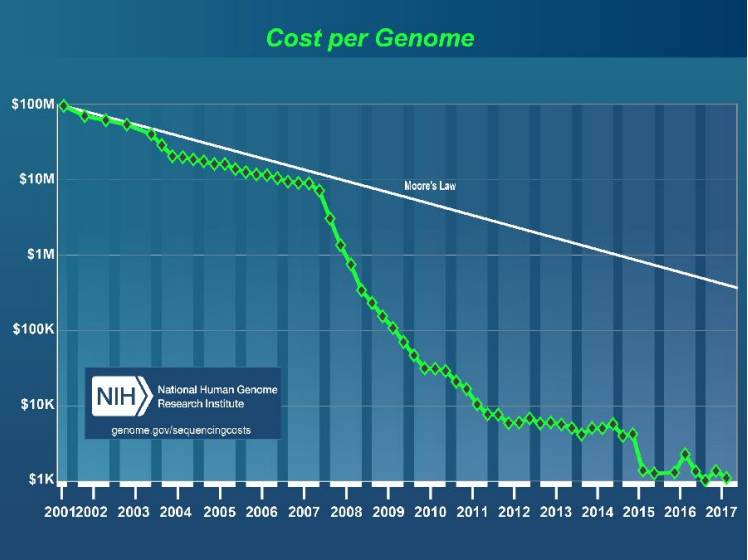
\includegraphics[scale=0.7]{poglavlja/9/slike/CostPerGenom.png}
\caption{Kretanje cene sekvencioniranja u poslednjih 17 godina}
\label{slika:X}
\end{figure}

\textbf{Referentni genom} je genom nastao na osnovu genoma 13 različitih pojedinaca. Ideja je bila da se napravi neki "prosečni" ljudski genom.



\begin{figure}[h!]
\centering
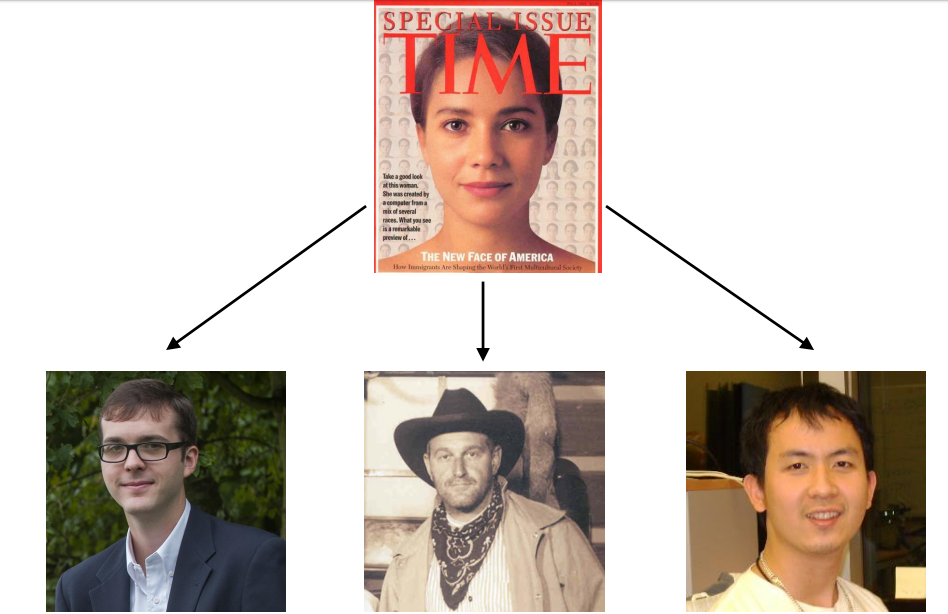
\includegraphics[scale=0.5]{poglavlja/9/slike/OdGenomaVrsteDoPersonalnih.png}
\caption{Prikaz grananja genoma vrste na više personalnih genoma}
\label{slika:X}
\end{figure}

U proseku, razlika između individualnog genoma je u oko 3 miliona mutacija.

\begin{figure}[h!]
\centering
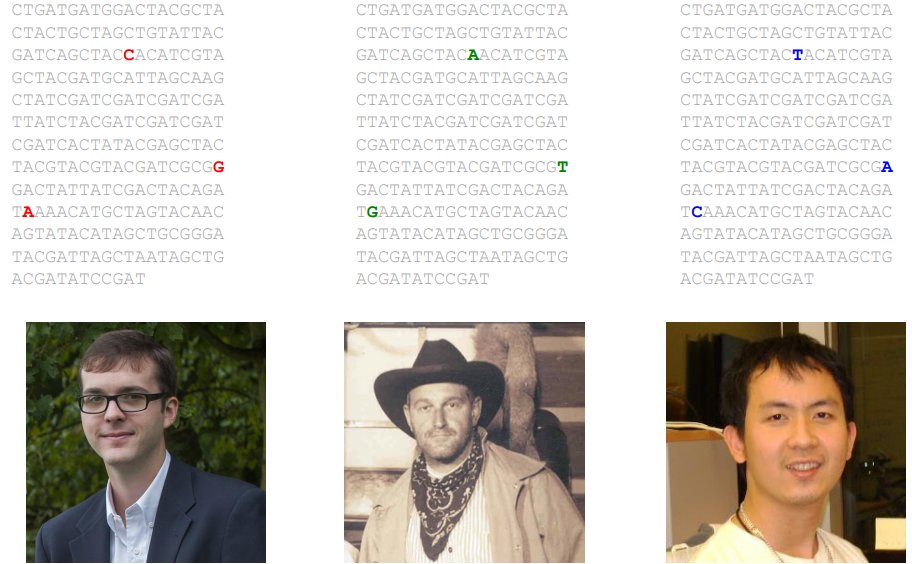
\includegraphics[scale=0.5]{poglavlja/9/slike/OdGenomaVrsteDoPersonalnih2.png}
\caption{Razlike u personalnim genomima}
\label{slika:X}
\end{figure}

Pitanje je kako možemo efikasno sastaviti individualne genome koristeći referentne. Možemo koristiti \textbf{asembliranje}, ali konstrukcija de Brojnovog grafa zahteva mnogo memorije. Možemo koristiti postojeću strukturu referentnog genoma kao pomoć u sekvencioniranju genoma pacijenta.
\begin{figure}[h!]
\centering
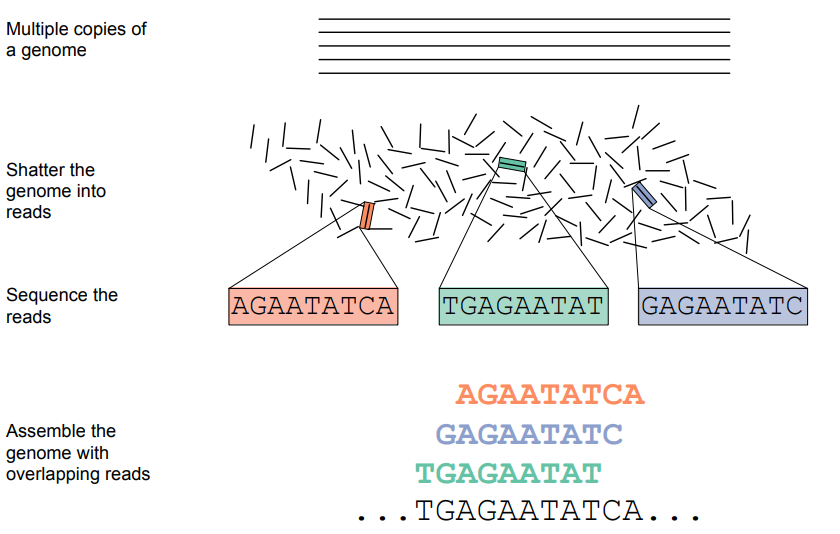
\includegraphics[scale=0.5]{poglavlja/9/slike/asembliranje.png}
\caption{Primer asembliranja}
\label{slika:X}
\end{figure}
\newpage
\textbf{Mapiranje očitavanja} predstavlja određivanje pozicije u referentnom genomu sa kojima svako očitavanje ima visoiku sličnost.

\begin{figure}[h!]
\centering
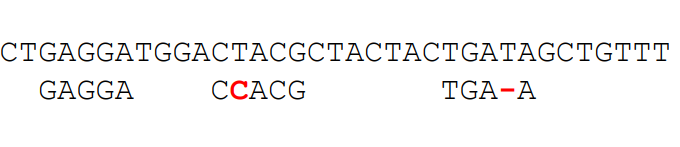
\includegraphics[scale=0.5]{poglavlja/9/slike/mapiranjeOcitavanja.png}
\caption{Primer mapiranja očitavanja; gornja niska predstavlja referentni genom, a donje očitavanja individualnog genoma}
\label{slika:X}
\end{figure}

\subsection{Egzaktno upativanje šablona}
Potrebno je pronaći gde se očitavanja egzaktno poklapaju sa referentnim genomom. Postoji jednostruko i višestruko uparivanje šablona.

\textbf{Problem jednostrukog uparivanja šablona:} \\
\indent \textbf{Ulaz:} Niske \textit{Pattern} i \textit{Genome}. \\
\indent \textbf{Izlaz:} Sve pozicije u niski \textit{Genome} gde se niska \textit{Pattern} pojavljuje kao podniska.
\\\\
\textbf{Problem višestrukog uparivanja šablona:} \\
\indent \textbf{Ulaz:} Kolekcija niski \textit{Patterns} i \textit{Genome}. \\
\indent \textbf{Izlaz:} Sve pozicije u niski \textit{Genome} gde se niske iz kolekcije \textit{Patterns} pojavljuju kao podniske.

\newpage
\subsection{Moguća rešenja}

Rešenje koje nam prvo pada na pamet je rešavanje problema grubom silom. Algoritam se sastoji u tome da se linearno krećemo kroz genom i proveravamo da li se dati šablon poklapa sa podniskom genoma iste dužine, koja počinje na toj poziciji.



\begin{figure}[h!]
\centering
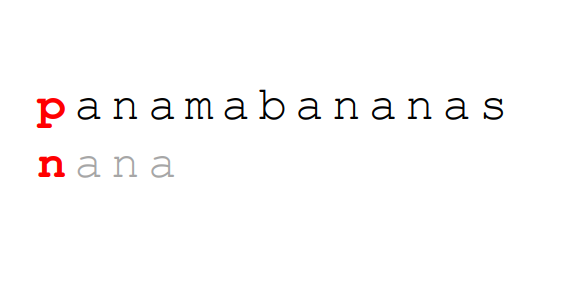
\includegraphics[scale=0.5]{poglavlja/9/slike/GrubaSilaGreska.png}
\caption{Uparivanje šablona grubom silom - nepoklapanje}
\label{slika:X}
\end{figure}

\begin{figure}[h!]
\centering
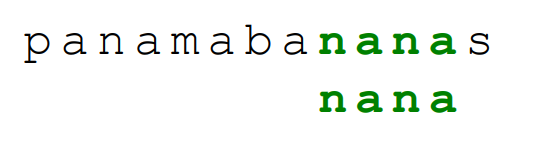
\includegraphics[scale=0.5]{poglavlja/9/slike/GrubaSilaPogodak.png}
\caption{Uparivanje šablona grubom silom - poklapanje}
\label{slika:X}
\end{figure}

Vreme izvršavanja algoritma u slučaju jednostrukog \textit{Pattern}-a je $O(|Genome| * |Pattern|)$, dok je u slučaju višestrukog \textit{Patterns}-a je $O(|Genome| * |Patterns|)$, gde je \textit{|Patterns|} suma dužina elemenata liste \textit{Patterns}. \\
Međutim, problem je u tome što genomi mogu biti veoma dugi. U slučaju ljudskog genoma (3 GB), ukupna dužina svih očitavanja može biti veća od 1 TB; kao rezltat toga, algoritam složenosti $O(|Genome| * |Patterns|)$ je previše spor.

\subsection{Sufiksna stabla}
Alternativni način je da paterne organizujemo u strukturu podataka poput usmerenog acikličnog grafa, koju nazivamo \textbf{Trie} i koja ima sledeće osobine:

\begin{itemize}
    \item Trie ima jedinstven čvor sa ulaznim stepenom nula, koji nazivamo koren
    \item Svaka grana Tria je obeležena jednim slovom
    \item Grane koje izlaze iz jednog čvora obeležene su različitim slovima
    \item Svaki sufiks neke niske dobija se nadovezivanjem slova duž neke putanje grafa, idući od korena naniže
    \item Svaka putanja stabla od korena do lista, ili do čvora sa izlaznim stepenom 0, predstavlja jedan element iz liste \textit{Patterns}
\end{itemize}

\begin{figure}[h!]
\centering
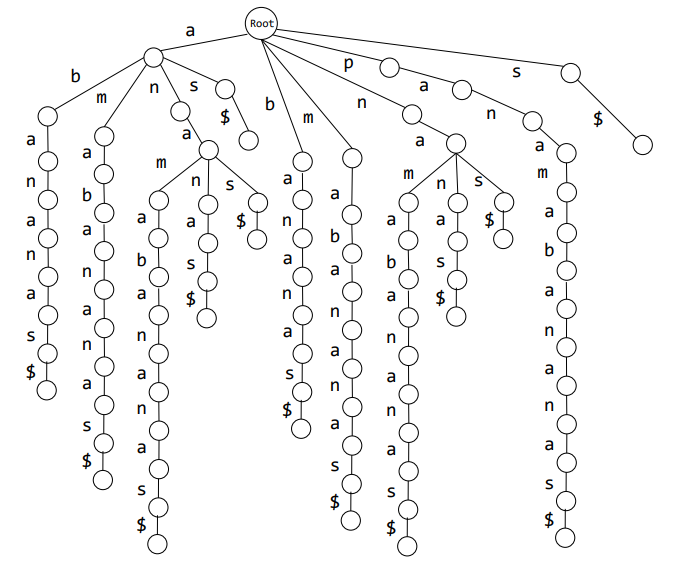
\includegraphics[scale=0.5]{poglavlja/9/slike/sufiksnoStabloNekompresovano.png}
\caption{Nekompresovano sufiksno stablo}
\label{slika:X}
\end{figure}


\begin{figure}[h!]
\centering
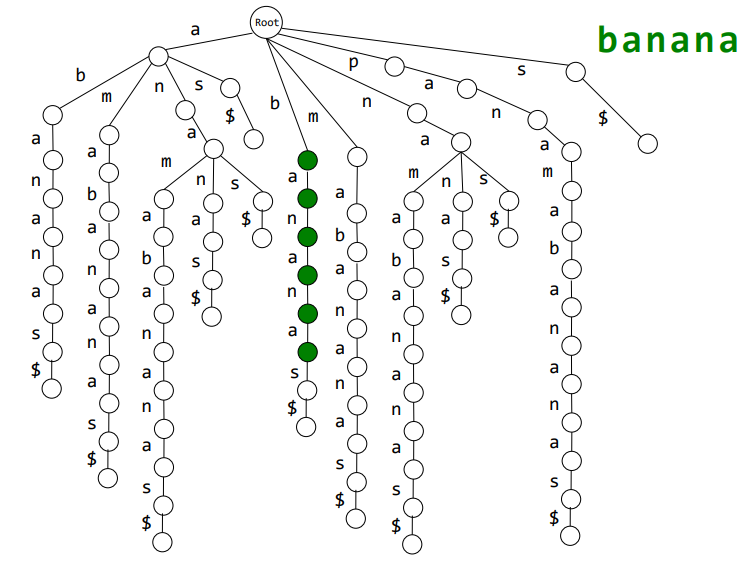
\includegraphics[scale=0.5]{poglavlja/9/slike/sufiksnoStabloNekompresovanoPogodak.png}
\caption{Nekompresovano sufiksno stablo - uspešno pronalaženje niske}
\label{slika:X}
\end{figure}

\begin{figure}[h!]
\centering
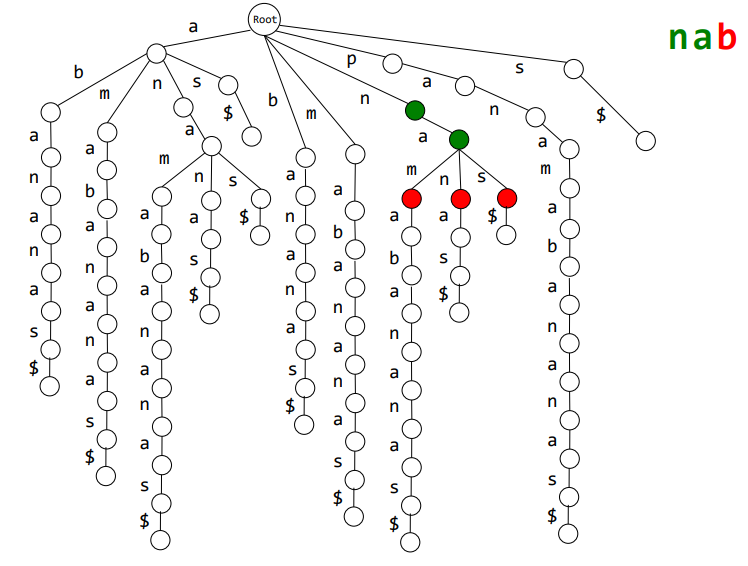
\includegraphics[scale=0.5]{poglavlja/9/slike/sufiksnoStabloNekompresovanoGreska.png}
\caption{Nekompresovano sufiksno stablo - neuspešno pronalaženje niske}
\label{slika:X}
\end{figure}


Ovim postupkom možemo utvrditi da li se pattern pojavljuje u genomu, ali ne i na kojoj poziciji. Za to moramo dodati još informacija u stablo. Na svakom listu dodamo početnu poziciju u niski Genome sufiksa koji se završava u tom listu.


\begin{figure}[h!]
\centering
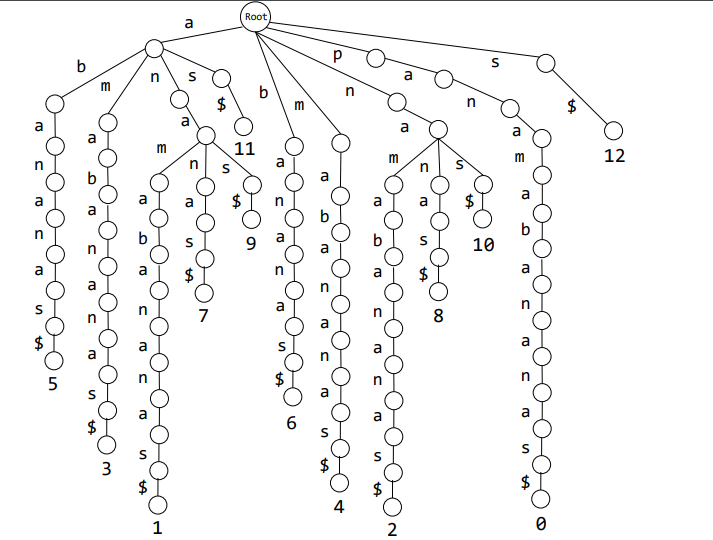
\includegraphics[scale=0.5]{poglavlja/9/slike/sufiksnoStabloNumerisaniPrefiksi.png}
\caption{Sufiksno stablo sa numerisanim prefiksima}
\label{slika:X}
\end{figure}

\clearpage
Sad se postavlja pitanje, kada pronađemo uparivanje, kako da znamo na kojoj poziciji se ono nalazi. To je sada lako, kada pronađemo uparivanje, nastavimo sa kretanjem naniže do lista, gde se nalazi pozicija odakle počinje pojavljivanje podniske. 

\begin{figure}[h!]
\centering
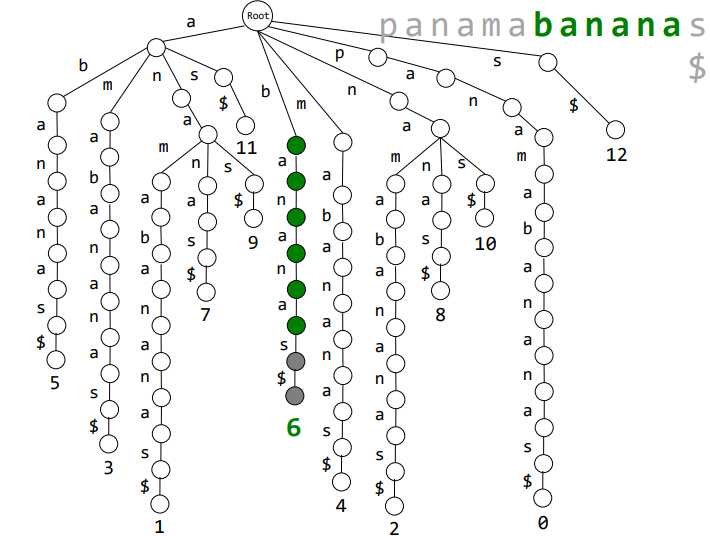
\includegraphics[scale=0.5]{poglavlja/9/slike/sufiksnoStabloNaciIndeksPocetka.png}
\caption{Primer nalaženja pozicije nakon uparivanja}
\label{slika:X}
\end{figure}

\begin{figure}[h!]
\centering
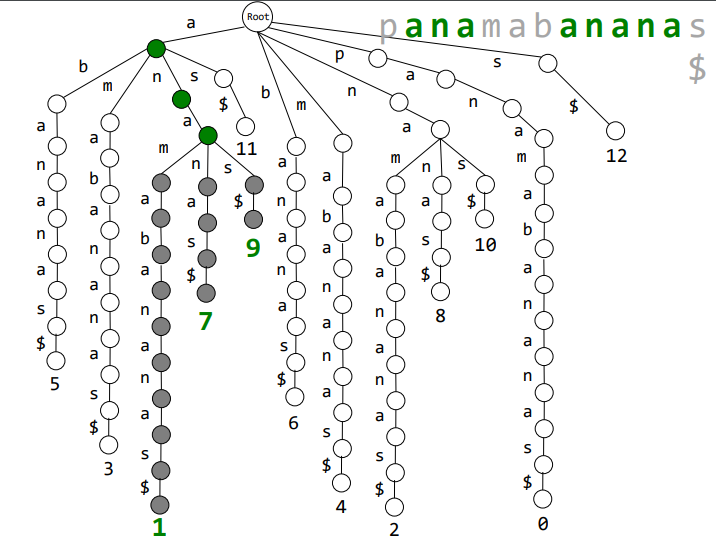
\includegraphics[scale=0.5]{poglavlja/9/slike/sufiksnoStabloNaciIndeksPocetkaVise.png}
\caption{Primer nalaženja pozicije nakon uparivanja - više poklapanja}
\end{figure}

\clearpage
Da bismo smanjili prostornu složenost, možemo kompresovati svaku putanju koja se ne grana u jednu granu. Ovakva struktura podataka naziva se \textbf{sufiksno stablo}.


Za svaku nisku \textit{Genome} važi da je ukupan broj čvorova manji od dvostruke dužine niske \textit{Genome}, odnosno $\# nodes < 2|Genome|.$
$$\# leaves = |Genome|$$
$$\# internal nodes < |Genome| - 1$$


\begin{figure}[h!]
\centering
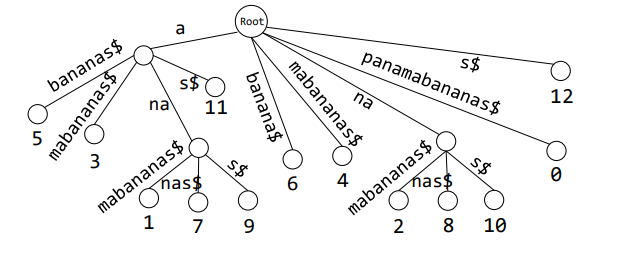
\includegraphics[scale=0.5]{poglavlja/9/slike/sufiksnoStabloKompresovano.png}
\caption{Kompresovano stablo}
\label{slika:X}
\end{figure}

\textbf{Prostorna i vremenska složenost}


Vremenska složenost: 
\begin{itemize}
\item O($|Genome|^2$) za konstrukciju sufiksnog stabla tako što se prvo konstruiše nekompresovano sufiksno stablo.
\item O($|Patterns|$) za nalaženje uparivanja.
\end{itemize}
Prostorna složenost:
\begin{itemize}
\item O($|Genome|^2$) za konstrukciju sufiksnog stabla tako što se prvo konstruiše nekompresovano sufiksno stablo.
\item O($|Patterns|$) za čuvanje sufiksnog stabla.
\end{itemize}




Postoje algoritmi sa linearnom prostornom i vremenskom složenošću.
Vremenska složenost: 
\begin{itemize}
\item O($|Genome|$) za konstrukciju sufiksnog stabla direktno.
\item O($|Patterns|$) za nalaženje uparivanja.
\item Ukupno O($|Genome|$ + $|Patterns|$)
\end{itemize}
Prostorna složenost:
\begin{itemize}
\item O($|Genome|^2$) za konstrukciju sufiksnog stabla direktno.
\item O($|Patterns|$) za čuvanje sufiksnog stabla.
\item Ukupno O($|Genome|$)
\end{itemize}

\section{Kompresija niski i Barouz-Vilerova transformacija}

Najveći problem koji se javlja sa prethodnom rešenjem je to što O-notacija ignoriše konstante, a najpoznatija implementacija sufiksnih stabala zahteva ~ 20 * |Genome| (npr. veličina humanog genoma je 3GB => 60 GB; i dalje unapređenje u odnosu na 1TB). Postavlja se pitanje da li možemo smanjiti faktor konstante. Odgovor nam daje kompresija genoma.

\subsection{Kompresija genoma}

Glavna ideja ovog rešenja jeste da se smanji količina memorije potrebna za čuvanje niske Genome. Za ovo su nam potrebne metode za kompresiju niske velikih dužina, što je naizgled sasvim drugačiji problem.

U ovom nekim genomima imamo nekoliko uzastopnih ponavljanjajedneaminokiseline(ranovi, runs): prvo uzastopna ponavljanja aminokiseline G, pa C i tako dalje), a u nekim imamo uzastopna ponavljanja nizova aminokiselina (ripitsi, repeats): prvo uzastopna ponavljanja GAC, pa CATT i tako dalje.

Prva ideja pri rešavanju ovog problema jeste da kodiramo dužine ranova.
\begin{figure}[h!]
\centering
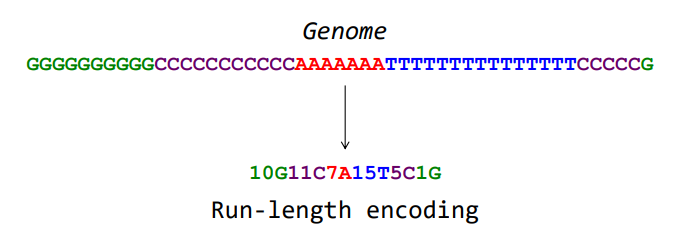
\includegraphics[scale=0.5]{poglavlja/9/slike/kompresijaGenoma.png}
\caption{}
\label{slika:X}
\end{figure}

Problem kod ovog pristupa jeste to što u genomu nema mnogo ranova. Međutim, ima mnogo ripita.
Postavlja se pitanje kako izvesti transformaciju ripita u ranove.
\begin{figure}[h!]
\centering
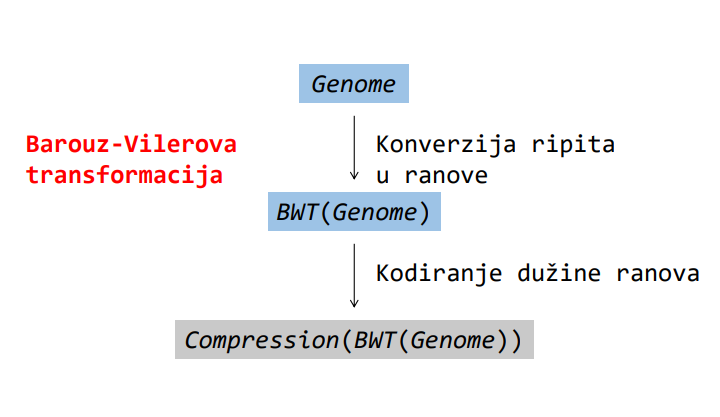
\includegraphics[scale=0.5]{poglavlja/9/slike/konversijaRipitaUranove.png}
\caption{}
\label{slika:X}
\end{figure}

Odgovor na ovo pitanje daje nam Varouz-Vilerova transformacija (BWT).


\begin{figure}[h!]
\centering
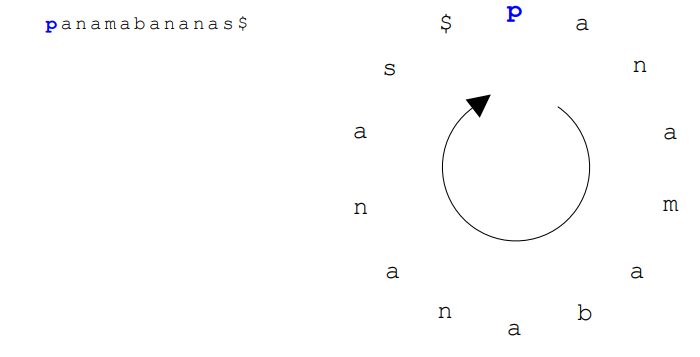
\includegraphics[scale=0.6]{poglavlja/9/slike/BWT.png}
\caption{}
\label{slika:X}
\end{figure}

\newpage

Ideja kod ovog algoritma je da se na početku formiraju sve ciklične rotacije date niske.

\begin{figure}[h!]
\centering
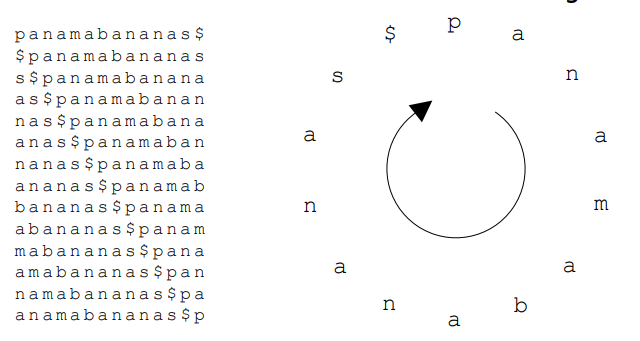
\includegraphics[scale=0.7]{poglavlja/9/slike/SveCiklicneRotacije.png}
\caption{Scenario sa 4 promene}
\label{slika:X}
\end{figure}

Zatim se vrši sortiranje svih dobijenih niski leksikografski (\$ je na početku).

\begin{figure}[h!]
\centering
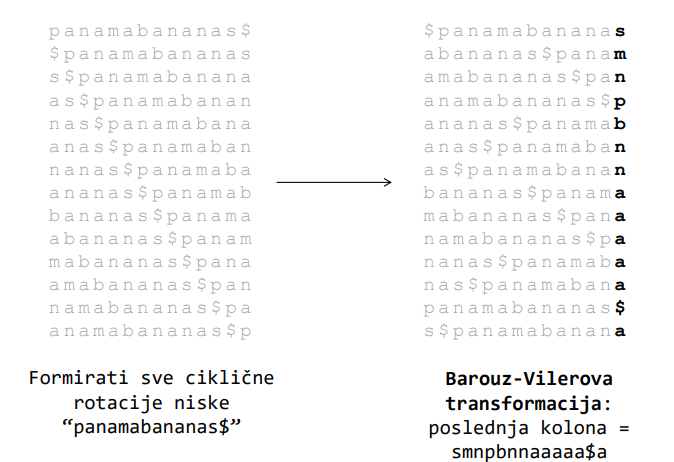
\includegraphics[scale=0.4]{poglavlja/9/slike/BWTPoslednjaKolona.png}
\caption{Pohlepno sortiranje}
\label{slika:X}
\end{figure}

Zatim posmatramo poslednju kolonu. Možemo primetiti da poslednja kolona sadrži veliki broj ranova. Međutim, isti slučaj je i sa prvom kolonom. Prvo ćemo se pozabaviti dekompresijom dobijene niska, pa ćemo se posle vratiti na ovo pitanje.


\section{Inverzna BWT}



\begin{figure}[h!]
\centering
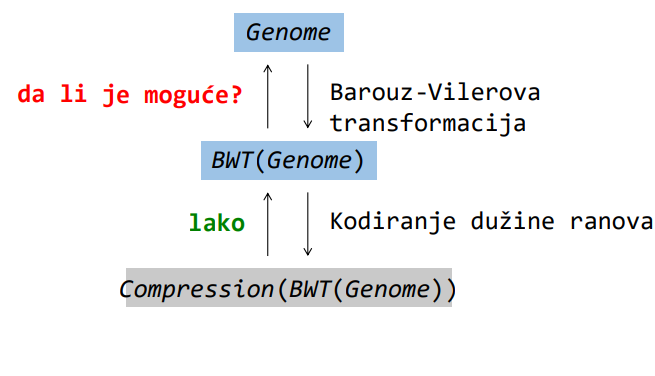
\includegraphics[scale=0.5]{poglavlja/9/slike/KakoDekompresiju.png}
\caption{}
\label{slika:X}
\end{figure}


Pogledajmo primer BWT-a za nisku \textit{banana}.


\begin{figure}[h!]
\centering
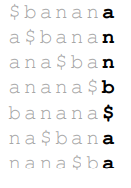
\includegraphics[scale=0.5]{poglavlja/9/slike/banana.png}
\caption{}
\label{slika:X}
\end{figure}


Ako sortiramo karaktere poslednje kolone “annb\$aa”, dobićemo prvu kolonu matrice. Na osnovu toga znamo 2-gramski sastav cirkularne niske \textit{banana\$}.

Srtiranjem niski dobijamo prve dve kolone matrice.

\begin{figure}[h]
\centering
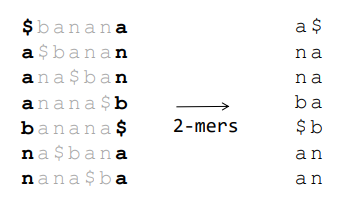
\includegraphics[scale=0.7]{poglavlja/9/slike/2-gramskiSastav.png}
\caption{}
\label{slika:X}
\end{figure}

Sada imamo dve kolone cikličnih niski. Zatim ponavljamo postupak - dodamo poslednju koju znamo, itd. Na kraju dobijamo rekonstruisanu celu matricu

\begin{figure}[h!]
\centering
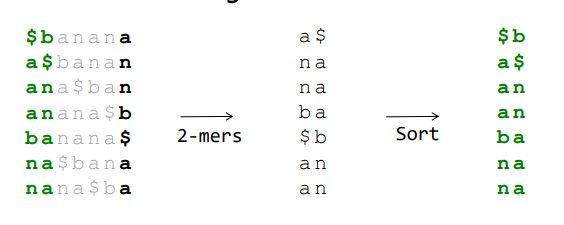
\includegraphics[scale=0.5]{poglavlja/9/slike/2-gramskiSastav2.png}
\caption{}
\label{slika:X}
\end{figure}

Nisku banana\$ dobijamo tako što uzmemo sve elemente iz prvog reda posle \$.
\newpage
\textbf{Prostorna složenost:}

Rekonstrukcija niske Genome na osnovu BWT(Genome) zahteva čuvanje |Genome| kopija niske Genome, što iznosi O($|Genome|^2$). Poboljšanje složenosti je moguće ako primetimo nešto.

\textbf{First-Last} svojstvo: k-to pojavljivanje simbola u FirstColumn i k-to pojavljivanje simbola u LastColumn odgovaraju istoj poziciji simbola u niski Genome.

\begin{figure}[h!]
\centering
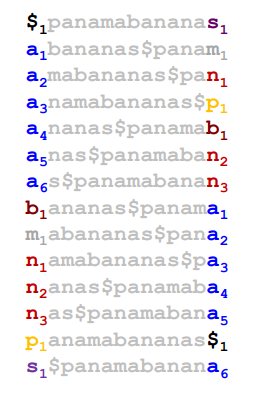
\includegraphics[scale=0.6]{poglavlja/9/slike/firstLast.png}
\caption{First-Last svojstvo}
\label{slika:X}
\end{figure}

\subsection{Efikasnija BWT dekompresija}

Krenemo od \$ (prvi u nizu cikličnih niski) u FirstColumn, vidimo koji je u LastColumn u tom redu, nađemo ga u FirstColumn, onda za taj nađemo koji je u tom redu u LastColumn, itd. U jednom trenutku ćemo doći do \$, u LastColumn i tada smo okrenuli ceo krug i rekonstruisali celu Genome nisku.
Prostorna složenost je 2|Genome| = O(|Genome|).


\subsection{Korišćenje BWT za uparivanje šablona}

Da se podsetimo, uparivanje šablona korišćenjem sufiksnih stabala zahtevalo je vremensku složenost od O(|Genome| + |Patterns|), prostorna O(|Genome|). Problem je bio što je sufiksno stablo tražilo 20 * |Genome| prostora.

Poboljšanje možemo dobiti ako umesto sufiksnog stabla budemo koristili BWT(Genome) kao strukturu podataka.

Krenemo od kraja niske koju tražimo i u FirstColumn tražimo taj karakter. Onda u LastColumn tražimo drugi od pozadi karakter od tih kojima je u FirstColumn kojima je u FirstColumn poslednji iz uzorka.

Zatim nađemo u FirstColumn gde su ti iz LastColumn i gledamo naredni karakter. Ako se poklapa sa trećim od pozadi nastavljamo nastavljamo dalje, ako nema ga. I tako dok ne pređemo ceo uzorak od kraja ka početku.

\begin{figure}[h!]
\centering
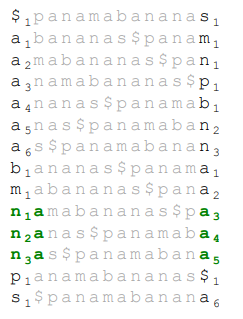
\includegraphics[scale=0.5]{poglavlja/9/slike/traziAnukraj1.png}
\caption{First-Last svojstvo}
\label{slika:X}
\end{figure}
\subsection{Pronalaženje uparenih šablona}


\begin{figure}[h!]
\centering
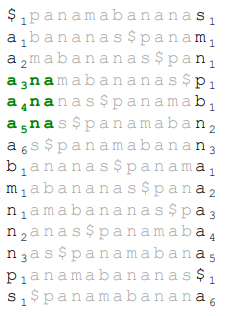
\includegraphics[scale=0.5]{poglavlja/9/slike/traziAnukraj2.png}
\caption{First-Last svojstvo}
\label{slika:X}
\end{figure}
\subsection{Pronalaženje uparenih šablona}

Problem višestrukog uparivanja šablona:\\
\textbf{Ulaz:} Kolekcija niski Patterns i niska Genome.\\
\textbf{Izlaz:} Sve pozicije u niski Genome gde se niske iz kolekcije Patterns pojavljuju kao podniske.

Treba da nađemo pozicije. BWT ne daje svoj podatak. Na primer, na gornjem promeru Ana se pojavljuje 3 puta, ali na kojim pozicijama?

Na kojim pozicijama se nalazi odredićemo pomoću sufiksnog niza.

Sufiksni niz je niz koji čuva početnu poziciju za svaki sufiks (niz karaktera u svakom redu matrice do simbola \$).


\begin{figure}[h!]
\centering
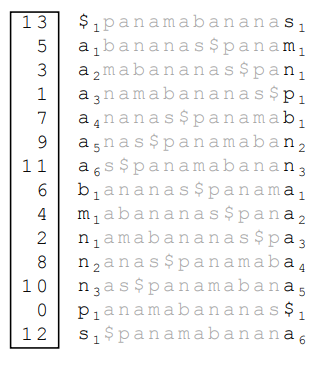
\includegraphics[scale=0.75]{poglavlja/9/slike/sufiksniNiz.png}
\caption{Sufiksni niz}
\label{slika:X}
\end{figure}

\newpage

Sa slike vidimo da se \textbf{ana} iz prethodnog primera pojavljuje na pozicijama 1, 7 i 9.

Prostorna složenost je $4 * |Genome|$ (ako koristimo 4B za cele brojeve kao elemente niza), što je bolje nego $20 * |Genome|$.

\section{Približno preklapanje}

Ponekad je nophodno pronaći približna uparivanja šablona.

\textbf{Ulaz:} Niska Pattern, niska Genome, ceo broj d (kod višestrukog uparivanja ulaz je kolekcija niski Patterns).
\textbf{Izlaz:} Sve pozicije niske Genome, gde se niska Pattern pojavljuje kao podniska sa najviše d razlika.

Traženje preklapanja radimo kao i pre, samo što sada prihvatamo i kad imamo različite karaktere (crvena slova na slici ispod), sve dok je broj razlika <= d.

\begin{figure}[h!]
\centering
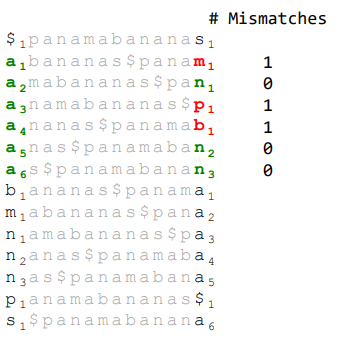
\includegraphics[scale=0.5]{poglavlja/9/slike/PribliznoPreklapanjeMissmatch.png}
\caption{Traženje približnog preklapanja za d = 1}
\label{slika:X}
\end{figure}
\newpage
Na kraju ovog primera pronašli smo 5 3-grama sa najviše jednim nepoklapanjem (pretpostavili smo da je d = 1).

\begin{figure}[h!]
\centering
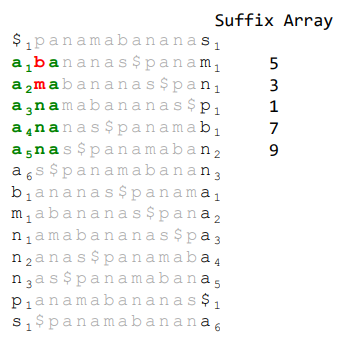
\includegraphics[scale=0.5]{poglavlja/9/slike/PribliznoPreklapanjeTrazenjeNiske.png}
\caption{Pozicije u genomu gde se javljaju približna preklapanja}
\label{slika:X}
\end{figure}

\section{Zadaci sa vezbi}

\setexamplecodestyle
\subsection{TrieConstruction}
%\lstinputlisting[language=Python]{poglavlja/9/kodovi/TrieConstruction.py}

\subsection{SufixReconstruction}
%\lstinputlisting[language=Python]{poglavlja/9/kodovi/SufixReconstruction.py}

\subsection{BWT}
%\lstinputlisting[language=Python]{poglavlja/9/kodovi/BWT.py}
